%% Placeholder for chapter on vector and functions

\noindent\textcircled{1} Geometry\\
-Vectors and vector spaces\\
-Norms\\
-Inner product\\

\noindent\textcircled{2} Projection\\
-On to subspace\\
-On to affine sets\\
-Non-Euclidean\\

\noindent\textcircled{3} Functions\\
-Functions and sets\\
-Linear and affine\\
-Gradients and Taylor approximations\\

\newpage

As mentioned in introduction, the 1st part of this course will focus on geometry. Linear algebra is the mathematical study of geometry in (arbitrary large) dimensions.

It turns out that your geometry xxx from $\reals^{2}$ to $\reals^{3}$(planes and space) is extremely helpful to conceive of large dimensional sets and understand operations on them.

Lots(but not all) of what we cover in the first few topics will repeat what you saw in your linear algebra course(Math 188/185).

\vspace{0.5cm}
\noindent Why repeat?

-Linear algebra in year 1, perhaps semester 1.

-It takes time xxx, to "get" linear algebra. If you are in this course, you are likely to come up a lot going forward.

-In your linear algebra course may have concentrate more on the "algebra" side of linear algebra rather than the geometry side. Our focus will be on the latter. E.g., $y-x^{2}=0$ is an algebraic relation but defines a geometric object(a parabola).

-If you took ECE216 with me you will see some familiar examples, and I encourage you to  connecting questions (perhaps after class as xxx all students took ECE216).

\newpage

\noindent\textbf{Vector}:A collection of numbers.
\begin{equation*}
x = \left[ \begin{array}{c} x_1 \\ x_2 \\ \vdots \\ x_n\end{array} \right].
\end{equation*}
where each $x_i \in \reals$ or $x_i \in \complex$. The length $n$ of the vector is also termed the "dimension" of the vector, which will subsequently be defined formally.

Our default will be a column vector as we describe above. Transpose x yields a row vector,   
\begin{equation*}
x^\trans = [ x_1 \ x_2 \ \ldots x_n].
\end{equation*}
and occasionally write as a list $(x_{1}, x_{2},\cdots,x_{n})$.  Note that a vector is not a set of numbers since order matters.

Also, we often need to work with a set(or list) of vectors,
\begin{equation*}
\{ \vecx{1}, \vecx{2}, \ldots, \vecx{m}\}
\end{equation*}
where $\vecx{i} \in \reals^n$, $i \in \{1, 2, \ldots, m\}$, $i \in [m] = \{1,2,\cdots,m\}$ and
$(\vecx{i})^\trans = [ \vecx[1]{i} \ \vecx[2]{i} \ \ldots \ \vecx[n]{i} ]$.  

Note: book not 100\% consistent, XXX

\vspace{0.5cm}
\noindent\textbf{Vector Space}

To this point a vector is just a lost of numbers.

To get to geometry, we need to define how to add pairs of vectors and how to scale vectors.

Addition: $u=v^{1}+v^{2}$, means $u_{i}=v_{i}^{1}+v_{i}^{2}$ for all $i\in [n]$.

Scaling: $u=av$,  means $u_{i}=v_{i}^{1}+v_{i}^{2}$ for all $i\in [n]$.

Linear combination: $\sum_{i=1}^{m} a_{i}v^{(i)}$

\begin{marginfigure}
	\centering
	\resizebox{7.5cm}{3cm}{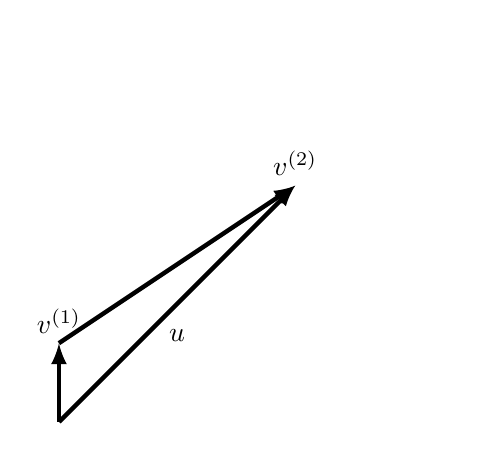
\begin{tikzpicture}
\draw [white, <->] (0,5) -- (0,0) -- (5,0);
\draw [-latex, ultra thick] (0,0) -- (0,1);
\draw [-latex, ultra thick] (0,0) -- (3,3);
\draw [-latex, ultra thick] (0,1) -- (3,3);
\node [above] at (0,1) {$v^{(1)}$};
\node [below] at (1.5,1.3) {$u$};
\node [above] at (3,3) {$v^{(2)}$};
\end{tikzpicture}}
	\caption{Add}
	\label{fig.2-1}
\end{marginfigure}
\begin{marginfigure}
	\centering
	\resizebox{7.5cm}{3cm}{\begin{tikzpicture}
\draw [white, <->] (0,5) -- (0,0) -- (5,0);
\draw [-latex, ultra thick] (0,0) -- (1.5,1.5);
\draw [-latex, ultra thick] (1.5,1.5) -- (3,3);
\node [above] at (0.75,0.75) {$v^{(1)}$};
\node [above] at (3,3) {$u=2v^{(1)}$};
\end{tikzpicture}}
	\caption{Scale}
	\label{fig.2-2}
\end{marginfigure}

Note that If $a=0$, then $u=av^{(1)}=0$.

\vspace{0.5cm}

With respect to the XXX at the origin can think of as xxx as a displacement(a move through the space) from the origin.

For any vector $v\in\reals$, $v=v-0$.

Note: XXX


Vector Space: a set of vectors that is closed under addition and scaling.

Formally we need following axioms:

Commutativity: $u+v=v+u$

Associativity: $(u+v)+w=u+(v+w)$

Distributivity: $a(u+v)=au+av$,\ $(a+b)u=au+bu$

Identity element of addition: $\exists 0\in \gamma$ s.t. $u+0=u$

Inverse elements of addition: $\exists -u\in \gamma$ s.t. $u+(-u)=0$

Identity element of scalar multiplication: $\exists a\in \reals\ \text{or}\ \complex$ s.t. $au=u$

In this course our focus is on $\reals^{n}$, i.e., finite-length vectors with real elements.

It is also useful to note that the geometric ideas could apply to lots of other spaces.\\
\textcircled{1} Finite-length complex vector\\
we need this esp for discussion of eigenvalues and eigenvectors. But also important examples in quantum computing.\\
\textcircled{2} $\infty$-length complex sequences(DT signals\&system)\\
\textcircled{3} Complex functions defined on real line(CT signals\&system)\\
\textcircled{4} Polynomials of degree at most n-1\\
$$P_{n-1}=\{P|p(t)=a_{n-1}t^{n-1}+a_{n-2}t^{n-2}+\cdots + a_{1}t+a_{0} \}$$
It can xxx linear combinations of polynomials and doesn't increase degree, so closed.\\
\textcircled{5} Sets of matrices(will discuss later)\\

Note: Some authors prefer “linear space" rather than "vector space" since elements of space are not always vectors in the sense of a list.

\vspace{0.5cm}

Span and subspace

If I give you a set of vectors, thinking of each as a displacement, anywhere you can get to via linear combinations is the "span" at the set.

If $S=\{v^{(1)}, v^{(2)}, \cdots ,v^{(m)}\}$, where each $v^{(i)}\in \reals^{n}$

Then span(S)$=\{\sum_{i=1}^{m} a_{i}v^{(i)}| a_{i}\in \reals ,\forall i\in [m]\}$

Example 1\\
Let $S=\{v^{(1)}\}=\left\{ 
\left[ 
\begin{array}{c} 
1 \\
1
\end{array}
\right]\right\}$

then
\begin{align*}
span(S)&=span({v^{(1)}})\\
&=\left\{\left[ 
	\begin{array}{c} 
	x \\
	y
	\end{array}
	\right]|x=y\right\}\\
&=\left\{a\left[ 
	\begin{array}{c} 
	1 \\
	1
	\end{array}
	\right]|a\in\reals\right\}
\end{align*}\\
\begin{marginfigure}
	\centering
	\resizebox{7.5cm}{3cm}{\begin{tikzpicture}
\draw [white, <->] (0,3) -- (0,0) -- (3,0);
\draw [-latex, ultra thick] (0,0) -- (1,1);
\draw [dashed,ultra thick] (-2,-2) -- (2,2);
\node [below right] at (0,0) {(0,0)};
\node [above left] at (1,1) {$v^{(1)}$};
\end{tikzpicture}}
	\caption{}
	\label{fig.2-3}
\end{marginfigure}


Example 2\\
$S=\{v^{(1)}, v^{(2)}\}=\left\{\left[ 
\begin{array}{c} 
1\\
1\\
0
\end{array}
\right],           
\left[ 
\begin{array}{c} 
1\\
-1\\
0
\end{array}
\right]
\right\}$

\begin{align*}
span(S)&=\{a_{1}v^{(1)}, a_{2}v^{(2)}|(a_{1}, a_{2})\in \reals_{2}\}\\
&=\left\{\left[ 
	\begin{array}{c} 
	x\\
	y\\
	0
	\end{array}
	\right] |x\in\reals , y\in\reals\right\}\\
&=\text{x-y plane}
\end{align*}\\
\begin{marginfigure}
	\centering
	\resizebox{7.5cm}{3cm}{\begin{tikzpicture}
\draw [<->] (0,4) -- (0,0) -- (4,0);
\draw [->] (0,0) -- (3,2);
\draw [dashed] (0,0) -- (-1.5,-1);
\draw [-latex, ultra thick] (0,0) -- (1.7,0.5);
\draw [-latex,ultra thick] (0,0) -- (0.8,-1);
\node [below] at (4,0) {x};
\node [below] at (3,2) {y};
\node [left] at (0,4) {z};
\node [above right] at (1.7,0.5) {$v^{(1)}$};
\node [below left] at (0.8,-1) {$v^{(2)}$};
\end{tikzpicture}}
	\caption{}
	\label{fig.2-4}
\end{marginfigure}


In fact, the span of a set of vectors is a "subspace" is a subset of the XXX vector space($\reals^{n}$ or $\complex^{n}$). XXXX properties of a vector space

Note: $0\in\reals_{n}$ always included since we can set all coefficients $a_{i}=0$ for all $i$.

Subspace is a "flat" that goes through the origin.

\vspace{0.5cm}
\noindent\textbf{Linear independent set}

$S=\{v^{(1)},\cdots , v^{(n)}\}$ is a linear, independent set if no element of $S$ can be expressed as a linear combination of the others.

The set $S$ is linearly independent if the only $a_{i}$ that satisfies

$\sum_{i=1}^{m}a_{i}v^{(i)}=0$ is if $a_{i}=0$ $\forall i\in [m]$

If this were not true, letting $l\in[m]$ be s.t. $a_{l}\neq 0$ would have
$$a_{l}v^{l}+\sum_{i\neq l} a_{i}v^{(i)}=0$$
$$v^{(l)}=\sum_{i\neq l}(\frac{-a_{i}}{a_{l}})v^{(i)}$$

Note that $a_{l}\neq 0$. So it is not linearly independent.

\vspace{0.5cm}
\noindent Importance of linearly independent

For any $u\in span(S)$ that is a unique choice of the $a_{i}$ in the expression
$u=\sum_{i=1}^{m} a_{i}v^{(i)}$, i.e., only one way to express.

\begin{marginfigure}
	\centering
	\resizebox{7.5cm}{3cm}{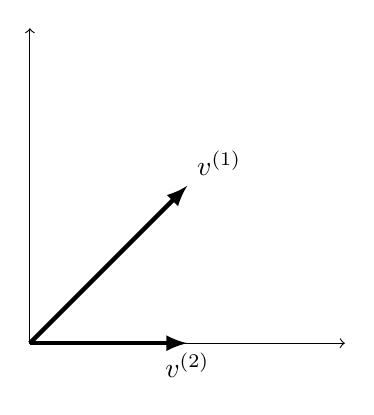
\begin{tikzpicture}
\draw [<->] (0,4) -- (0,0) -- (4,0);
\draw [-latex, ultra thick] (0,0) -- (2,2);
\draw [-latex,ultra thick] (0,0) -- (2,0);
\node [above right] at (2,2) {$v^{(1)}$};
\node [below] at (2,0) {$v^{(2)}$};
\end{tikzpicture}}
	\caption{}
	\label{fig.2-4}
\end{marginfigure}
\begin{marginfigure}
	\centering
	\resizebox{7.5cm}{3cm}{\begin{tikzpicture}
\draw [<->] (0,5) -- (0,0) -- (5,0);
\draw [-latex, ultra thick] (0,0) -- (2,2);
\draw [-latex,ultra thick] (2,2) -- (4,2);
\draw [dashed,ultra thick] (-2,2) -- (5,2);
\node [below] at (5,0) {$u_{1}$};
\node [left] at (0,5) {$u_{2}$};
\node [above right] at (4,2) {$a_{1}v^{(1)}$};
\node [below right] at (2,2) {$a_{2}v^{(2)}$};
\end{tikzpicture}}
	\caption{}
	\label{fig.2-4}
\end{marginfigure}

$v^{(1)}= 
\left[ 
\begin{array}{c} 
1 \\
0
\end{array}
\right]$
,
$v^{(1)}= 
\left[ 
\begin{array}{c} 
1 \\
1
\end{array}
\right]$

No redundancy is representation.

observe: it did have redundancy in S. For example,

$S=\left\{\left[ 
\begin{array}{c} 
1\\
0
\end{array}
\right],           
\left[ 
\begin{array}{c} 
1\\
1
\end{array}
\right],
\left[ 
\begin{array}{c} 
0\\
1
\end{array}
\right]
\right\}$

can always shrink S by removing elements to get a linearly independent set. Such an irreducible or linearly independent set can serve as a basis for span(S).

Any largest linearly independent subset of $S=\{v^{(1)},\cdots , v^{(m)}\}$,$B=\{v^{(1)},\cdots , v^{(k)}\}$, $k\leq m$ is a basis for span(S), and the dimension of span(S), dim(span(S))=k.


Example

$v^{(1)}= 
\left[ 
\begin{array}{c} 
1 \\
1 \\
1
\end{array}
\right]$,
$v^{(2)}= 
\left[ 
\begin{array}{c} 
1 \\
2 \\
0
\end{array}
\right]$,
$v^{(3)}= 
\left[ 
\begin{array}{c} 
1 \\
3 \\
1
\end{array}
\right]$

an linearly independent spanning set form a basis for

$span\left(\{v^{(1)},v^{(2)}, v^{(3)}\right\}=\reals^{3}$

But, if swap $v^{(3)}= 
\left[ 
\begin{array}{c} 
3 \\
4 \\
2
\end{array}
\right]
=2v^{(1)}+v^{(2)}$

Then $\left(v^{(1)},v^{(2)}, v^{(3)}\right)$ is not a basis, and it need to be reduced to:

$span\left(\{v^{(1)},v^{(2)}\}\right)=span\left(\{v^{(1)},v^{(2)}\}\right)=span\left(\{v^{(1)},v^{(2)}\}\right)=span(S)$

We can prove that each a basis for span(S) all have same coordinates.

Example

Perhaps most familiar basis is the "standard" basis

$v^{(1)}= 
\left[ 
\begin{array}{c} 
1 \\
0 \\
0 \\
\vdots
\end{array}
\right]$,
$v^{(2)}= 
\left[ 
\begin{array}{c} 
0 \\
1 \\
0 \\
\vdots
\end{array}
\right]$, $\cdots$,
$v^{(n)}= 
\left[ 
\begin{array}{c} 
0 \\
0 \\
\vdots \\
1 
\end{array}
\right]$


often see "e" for standard basis, i.e., $e^{(i)}=v^{(i)}$.

Note that our book uses $e_{i}$ for $e^{(i)}$.

\vspace{0.5cm}
\noindent\textbf{Norms}: Another important property, idea of distance on length

Familiar: Euclidean distance 

But not only notion of distance. E.g. walking through downtown Toronto or NYC. Blocks you walk along the shortest park.

figure here

So, multiple sense of distance, a sense of distance for a vector is a "norm", some properties on norm must satisfy.

A norm $\Vert\cdot\Vert$ is a function such that $\Vert\cdot\Vert : \gamma\mapsto\reals$
and satisfies

(a)$\Vert v \Vert\geq 0$, $\forall v\in \gamma$, and $\Vert v \Vert=0$ iff $v=0$.

(b)$\Vert u+v \Vert\leq \Vert u \Vert+\Vert v \Vert$, $\forall u, v\in \gamma$.

(c)$\Vert au \Vert= \vert a\vert\Vert u \Vert$, $\forall a\in\reals, u\in\gamma$

Note:$\gamma$ can be either $\reals$ or $\complex$, if $\gamma\in\complex$ we should have $a\in\complex$ in (c).

a family of norms but will come up after are:

$L_{p}$ norm:

$$\Vert x\Vert_{p}=(\sum_{k=1}^{n}\vert x_{k}\vert^{p})^{1/p}, 1\leq p\leq\infty$$

$L_{2}$ norm: Euclidean length

$$\Vert x\Vert_{2}=\sqrt{\sum_{k=1}^{n}\vert x_{k}\vert^{2}}$$

$L_{1}$ norm:

$$\Vert x\Vert_{1}=\sum_{k=1}^{n}\vert x_{k}\vert$$

$L_{\infty}$ norm:

$$\Vert x\Vert_{\infty}=\lim_{p\to\infty}\Vert x_{k}\Vert_{p}=\max_{k\in [n]} \vert x_{k}\vert$$


Length is a notion of "size"

A natural notion of its "size" of a set is the number of non zero XXX

i.e., carnality of non-zero support

$$card(x)=\sum_{k=1}^{n}\mathbb{1}_{x_{k}\neq 0}$$

Sometimes it is called "$L_{0}$" $norm \Vert x\Vert_{0}$ since

$$card(x)=\lim_{p\to 0}(\sum_{k=1}^{n}\vert x_{k}\vert^{p})^{p}$$

But not a norm (so this terminology is inaccurate). E.g., it doesn't satisfy property (c),

$$card(2x)=card(x)\neq 2card(x)$$


To visualize a norm we often plot it unit norm-ball

$$\beta_{p}=\{x|\Vert x\Vert_{p}\leq 1\}$$

$L_{2}$

\begin{marginfigure}
	\centering
	\resizebox{7.5cm}{3cm}{%% page 15
%% fig 1
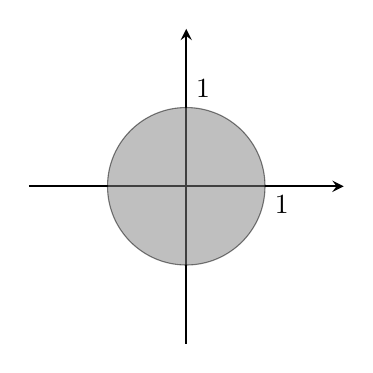
\begin{tikzpicture}
\draw[thick,-stealth] (-2, 0) -- (2, 0);
\draw[thick,-stealth] (0, -2) -- (0, 2);

\filldraw[fill=gray, draw=black, opacity=0.5] (0,0) circle [radius=1];
\node [below right] at (1, 0) {1};
\node [above right] at (0, 1) {1};
\end{tikzpicture}}
	\caption{}
	\label{}
\end{marginfigure}

$L_{1}$ : $\{x|\vert x_{1}\vert\leq 1\}$

\begin{marginfigure}
	\centering
	\resizebox{7.5cm}{3cm}{%% page 15
%% fig 2
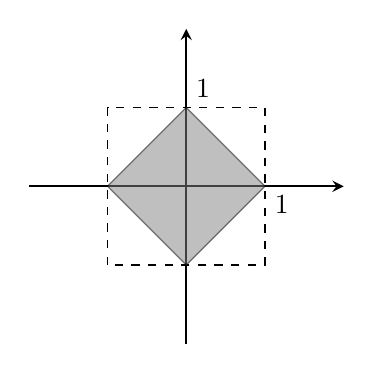
\begin{tikzpicture}
\draw[thick,-stealth] (-2, 0) -- (2, 0);
\draw[thick,-stealth] (0, -2) -- (0, 2);

\draw[dashed] (-1, -1) rectangle (1, 1);
\filldraw[draw=black, fill=gray, opacity=0.5] (-1, 0) -- (0, 1) -- (1, 0) -- (0, -1) -- (-1, 0);
\node [below right] at (1, 0) {1};
\node [above right] at (0, 1) {1};
\end{tikzpicture}
}
	\caption{}
	\label{}
\end{marginfigure}

(a) First see inside the box, clearly $\vert x_{1}\vert\leq 1$ and $\vert x_{2}\vert\leq 1$

(b) Look at the position we want, $x_{1}+x_{2}\leq 1$, i.e., $x_{2}\leq 1-x_{1}$

(c) Rest by symmetry


$L_{\infty}$ : $\{x|\max\{\vert x_{1}\vert, \vert x_{2}\vert\} \leq 1\}$

\begin{marginfigure}
	\centering
	\resizebox{7.5cm}{3cm}{%% page 15
%% fig 3
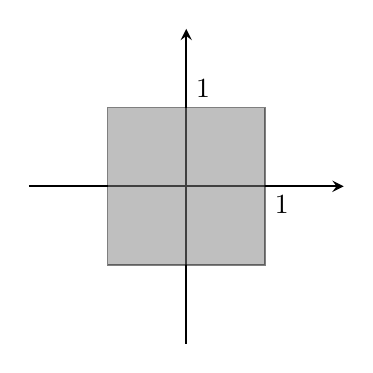
\begin{tikzpicture}
\draw[thick,-stealth] (-2, 0) -- (2, 0);
\draw[thick,-stealth] (0, -2) -- (0, 2);

\filldraw[fill=gray, draw=black, opacity=0.5] (-1, -1) rectangle (1, 1);
\node [below right] at (1, 0) {1};
\node [above right] at (0, 1) {1};
\end{tikzpicture}
}
	\caption{}
	\label{}
\end{marginfigure}


what about "$L_{0}$"? $\{x|card(x)\leq 1\}$

\begin{figure}
	\centering
	\resizebox{7.5cm}{3cm}{%% page 15
%% fig 4
\begin{tikzpicture}
\draw[thick,-stealth] (-2, 0) -- (2, 0);
\draw[thick,-stealth] (0, -2) -- (0, 2);

\draw (-1, 0) -- (1, 0)node[below]{1};
\draw (0, -1) -- (0, 1)node[right]{1};

\fill (0, 1) circle (1pt);
\fill (1, 0) circle (1pt);
\fill (0, -1) circle (1pt);
\fill (-1, 0) circle (1pt);
\end{tikzpicture}}
	\caption{}
	\label{}
\end{figure}

Not much of a "ball"


To visualize a bit more look at "level sets" of the norm balls.

$\{x|\vert x\vert=c \}$, see for $c=\frac{1}{2}, 1, 2$

$L_{1}$

\begin{marginfigure}
	\centering
	\resizebox{7.5cm}{3cm}{%% page 16
%% fig 1
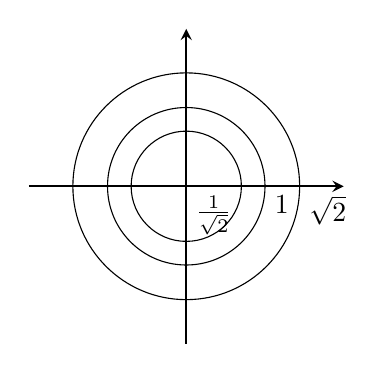
\begin{tikzpicture}
\draw[thick,-stealth] (-2, 0) -- (2, 0);
\draw[thick,-stealth] (0, -2) -- (0, 2);

\draw (0,0) circle [radius=0.7];
\node [below left] at (0.7, 0) {$\frac{1}{\sqrt 2}$};

\draw (0,0) circle [radius=1];
\node [below right] at (1, 0) {1};

\draw (0,0) circle [radius=1.44];
\node [below right] at (1.44, 0) {$\sqrt 2$};

\end{tikzpicture}
}
	\caption{}
	\label{}
\end{marginfigure}

$L_{2}$

\begin{marginfigure}
	\centering
	\resizebox{7.5cm}{3cm}{%% page 16
%% fig 2
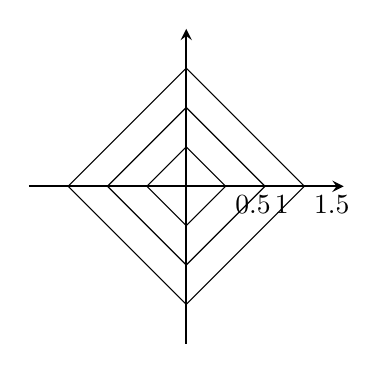
\begin{tikzpicture}
\draw[thick,-stealth] (-2, 0) -- (2, 0);
\draw[thick,-stealth] (0, -2) -- (0, 2);

\draw (-0.5, 0) -- (0, 0.5) -- (0.5, 0) -- (0, -0.5) -- (-0.5, 0);
\node [below right] at (0.5, 0) {0.5};

\draw (-1, 0) -- (0, 1) -- (1, 0) -- (0, -1) -- (-1, 0);
\node [below right] at (1, 0) {1};

\draw (-1.5, 0) -- (0, 1.5) -- (1.5, 0) -- (0, -1.5) -- (-1.5, 0);
\node [below right] at (1.5, 0) {1.5};
\end{tikzpicture}

}
	\caption{}
	\label{}
\end{marginfigure}

$L_{\infty}$

\begin{marginfigure}
	\centering
	\resizebox{7.5cm}{3cm}{%% page 16
%% fig 3
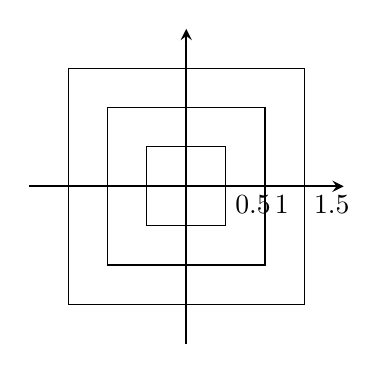
\begin{tikzpicture}
\draw[thick,-stealth] (-2, 0) -- (2, 0);
\draw[thick,-stealth] (0, -2) -- (0, 2);

\draw (-0.5, -0.5) rectangle (0.5, 0.5);
\node [below right] at (0.5, 0) {0.5};

\draw (-1, -1) rectangle (1, 1);
\node [below right] at (1, 0) {1};

\draw (-1.5, -1.5) rectangle (1.5, 1.5);
\node [below right] at (1.5, 0) {1.5};
\end{tikzpicture}
}
	\caption{}
	\label{}
\end{marginfigure}


Why might we be interested in different norms?


Ex: Later see applications in optimal control XXX want to meet a XXX objective (move a XXX from point a to XXX point b) while minimizing some resources $\rightarrow$ XXX will be XXX min a norm XXX XXX XXX 


$L_2$ $\rightarrow$ get min energy solution

$L_1$ $\rightarrow$ get a sparse solution not many forms of jet, useful when "XXX up" overhead

$L_\infty$ all uses of resource will be equal in XXX "XXX -XXX " XXX in XXX XXX

\vspace{0.5cm}
\noindent\textbf{Inner Products}

Final concept in geometry is angles which XXX to concept of inner product between elements of a vector space.

The "standard" inner product in $\reals_{n}$ (aka dot/scalar product)

$$x^{\trans}y=\sum_{k=1}^{n}x_{k}y_{k}$$

More general denote an inner product as $\langle x,y\rangle$

Definition: Any inner product on a (real) vector space $\Omega$ maps a pair of elements $x, y\in\Omega$ into the scalar, that is, $\langle \cdot,\cdot\rangle:\Omega\times\Omega\mapsto\reals$

For any $x, y, z\in\Omega$ and $a\in\reals$, the following holds:

$\langle x,y\rangle\geq 0$ and $\langle x,y\rangle=0$ iff $x=0\in\Omega$

$\langle x+y,z\rangle=\langle x,z\rangle+\langle y,z\rangle$

$\langle ax,y\rangle=a\langle x,y\rangle$

$\langle x,y\rangle=\langle y,x\rangle$


Note:
The above change slightly in complex vector space, e.g., $\langle x,y\rangle=\overline{\langle y,x\rangle}$

The concept we develop apply beyond list vectors in $\reals_{n}$ or $\complex_{n}$, e.g., space of polynomials or of XXX, but our focus will be $\reals_{n}$ and $\complex_{n}$.

Let's connect to angle now.

\begin{marginfigure}
	\centering
	\resizebox{7.5cm}{3cm}{%% page 18
\begin{tikzpicture}
\coordinate (O) at (0, 0);
\coordinate (A) at (4, 2);
\coordinate (B) at (1, 2);

\draw [ -stealth] (O) -- (A)node[below]{$x$};
\draw [ -stealth] (O) -- (B)node[above]{$y$};

\draw[dashed, -stealth] ($(O)!(B)!(A)$) -- (B)node[above, midway]{$\vec e$};

\draw [ -stealth] (O) -- ($(O)!(B)!(A)$)node[below right]{$x^{'}$};

\draw (A) -- (O) -- (B)
pic [draw= black, angle radius= 0.5cm, "$\theta$"] {angle = A--O--B};
\end{tikzpicture}
}
	\caption{}
	\label{}
\end{marginfigure}

Note: In above picture $x, y\in\reals_{n}$ but since $dim{span({x, y})}=2$ (assuming x and y are not co-linear). The familiar picture in $\reals_{2}$ shall holds.

Since we know that $\vert\cos\theta\vert <1$ XXX give

$$\vert\langle x,y\rangle\vert =\vert x^{\trans}y\vert \leq \Vert x\Vert_{2} \Vert y\Vert_{2}$$

Cauchy-Schwartz relates inner product(angle) to norms(length)

Holds for the inner products, not just in $\reals_{n}$

But can also related $\vert\langle x,y\rangle\vert$ to the norms (not $L_{2}$) via a generalization, "Holder's inequality"

$\vert x^{\trans}y\vert\leq \sum_{k=1}^{n}\vert x_{k}y_{k}\vert \leq \Vert x\Vert_{p}\Vert y\Vert_{q}$, for any $p, q\geq 1$ such that $1/p+1/q=1$

If $p=q=2$, get c-s

If $p=1$, $q=\infty$, get $\vert x^{\trans}y\vert\leq \Vert x\Vert_{1}\Vert y\Vert_{\infty}=(\sum_{k=1}^{n}\vert x_{k}\vert)(\max_{k\in [n]}x_{k})$



A second important connection of inner product and norm is that

$$\Vert x\Vert_{2}=\sqrt{x^{\trans} x}=\langle x,x\rangle$$

The $L_{2}$ norm is "induced" by the XXX inner product.

In fact, any inner product induces a norm (by the properties of inner product)

However, there are norms that are not induced by any inner product, e.g., $L_{1}$ and $L_{\infty}$.

Inner product space more special structure than a "normed" vector space.

\begin{marginfigure}
	\centering
	\resizebox{7.5cm}{3cm}{% page 19
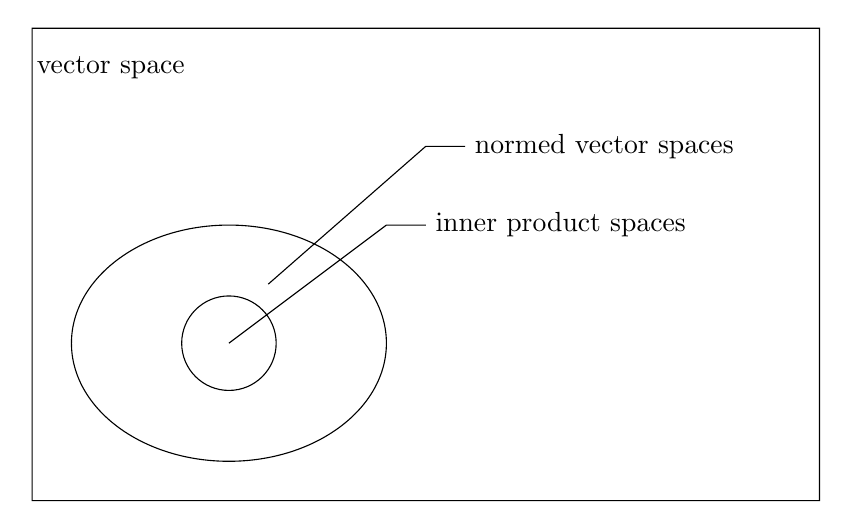
\begin{tikzpicture}
    \path 
        (0, 0) rectangle (10, 6) [draw]
        (1, 5.5) node {vector space}

        (2.5,2) coordinate (A) node[below] { } ellipse (2 and 1.5) [draw]
        
        coordinate (temp) at (2.5, 2) ellipse (0.6 and 0.6) [draw]
        (temp) +(0.5, 0.75) coordinate (B) node[below left] { } -- (5, 4.5) -- (5.5, 4.5) node[right]{normed vector spaces}

        (A) -- (4.5, 3.5) -- (5, 3.5) node[right]{inner product spaces} ;

\end{tikzpicture}
}
	\caption{}
	\label{}
\end{marginfigure}

Note: There are also spaces with a sense of length (a "metric"). Those are not vector spaces (it can't add and scale elements). Those are "metric" spaces.

\vspace{0.5cm}
\noindent\textbf{Angles between vectors}

Important XXX: since by Cauchy-Schwartz $\frac{\vert \langle x,y\rangle\vert}{\Vert x\Vert \Vert y\Vert}\leq 1$

(a) If $\vert\cos\theta\vert = +1$, then $\theta 0^{\circ}$ or $180^{\circ}$. x and y are "co-linear", and $\vert\langle x,y\rangle\vert=\Vert x\Vert \Vert y\Vert$

\begin{marginfigure}
	\centering
	\resizebox{7.5cm}{3cm}{%% page 20
%% fig 1
\begin{tikzpicture}
\draw [white, <->] (0, 5) -- (0, 0) -- (5, 0);
\draw [-latex, ultra thick] (0, 0) -- (2, 2);
\node [below] at (3, 2) {$x$};
\node [below] at (2, 2) {$\cos e = 1$};
\draw [-latex, ultra thick] (2, 2) -- (4, 4);
\node [below] at (5, 4) {$y$};
\end{tikzpicture}
}
	\caption{}
	\label{}
\end{marginfigure}

\begin{marginfigure}
	\centering
	\resizebox{7.5cm}{3cm}{%% page 20
%% fig 2
\begin{tikzpicture}
\draw [white, <->] (0, 5) -- (0, 0) -- (5, 0);
\draw [-latex, ultra thick] (2, 2) -- (0, 0);
\node [below] at (1, 0) {$y$};
\filldraw[black] (2, 2) circle (2pt) node[anchor=west] {$\cos e = -1$};
\draw [-latex, ultra thick] (2, 2) -- (4, 4);
\node [above] at (5, 4) {$x$};
\end{tikzpicture}

}
	\caption{}
	\label{}
\end{marginfigure}

(b) Perhaps more important if $\vert\cos\theta\vert = 0$, then $\theta 90^{\circ}$, and $\frac{\vert\langle x,y\rangle\vert}{\Vert x\Vert \Vert y\Vert}=0$, or equivalently, $\langle x,y\langle=0$ asumming $x\neq 0$ and $y\neq 0$

\begin{marginfigure}
	\centering
	\resizebox{7.5cm}{3cm}{%% page 20
%% fig 3
\def\RightAngle[size=#1](#2,#3,#4){%
 \draw ($(#3)!#1!(#2)$) -- 
       ($($(#3)!#1!(#2)$)!#1!90:(#2)$) --
       ($(#3)!#1!(#4)$);
 \path (#3) --
 ($($(#3)!#1!(#2)$)!#1!90:(#2)$);
}
\begin{tikzpicture}
\coordinate (A) at (0, 2);
\coordinate (B) at (5, 2);
\coordinate (C) at (1, 0);

\draw [white, <->] (0, 5) -- (0, 0) -- (5, 0);

\draw [-latex, ultra thick] (C) -- (A);
\node [below] at (0, 3) {$x$};

\draw [-latex, ultra thick] (C) -- (B);
\node [below] at (4, 1) {$y$};

%% right angle
\RightAngle[size=10pt](B,C,A);

\end{tikzpicture}
}
	\caption{}
	\label{}
\end{marginfigure}

$\theta$ is a "right" angle, and x, y are orthogonal vectors.

(c) If $\vert \theta\vert <90^{circ}$ ,then $\cos\theta >0$. So $\langle x,y\rangle >0$ on "acute angle".

\begin{marginfigure}
	\centering
	\resizebox{7.5cm}{3cm}{%% page 20
%% fig 4
\begin{tikzpicture}
\draw [<-] (0, 5) -- (0, -1);
\draw [->] (-1, 0) -- (5, 0);

\draw [-latex, ultra thick] (0, 0) -- (5, 0);
\node [below] at (5, 0) {$x$};

\draw [-latex, ultra thick] (0, 0) -- (3, 3);
\node [below right] at (3, 3) {$y$};

\draw (1, 0) coordinate (A) -- (0, 0) coordinate (B) -- (1, 1) coordinate (C)
pic [draw= black, angle radius= 1cm] {angle};
\node [below right] at (1, 0.5) {$o$};
\end{tikzpicture}
}
	\caption{}
	\label{}
\end{marginfigure}

\begin{marginfigure}
	\centering
	\resizebox{7.5cm}{3cm}{%% page 20
%% fig 5
\begin{tikzpicture}
\draw [<-] (0, 5) -- (0, -1);
\draw [->] (-5, 0) -- (5, 0);

\draw [-latex, ultra thick] (0, 0) -- (5, 0);
\node [below] at (5, 0) {$x$};

\draw [-latex, ultra thick] (0, 0) -- (-3, 3);
\node [below right] at (-3, 3) {$y$};

\draw (1, 0) coordinate (A) -- (0, 0) coordinate (B) -- (-1, 1) coordinate (C)
pic [draw= black, angle radius= 1cm] {angle};
\node [below right] at (1, 1) {$o$};
\end{tikzpicture}}
	\caption{}
	\label{}
\end{marginfigure}

wheres if $\vert \theta\vert >90^{circ}$, so $\langle x,y\rangle <0$ on "abluse angle".

\vspace{0.5cm}
\noindent\textbf{Orthogonality}

A set of vectors $S=\{x^{(1)}, x^{(2)},\cdots, x^{(n)}\}$ is mutually orthogonal if $\langle x^{(i)},x^{(j)}\rangle =0$, $\forall i\neq j$
					
Such sets have nice property that the elements of S are linearly independent and so provide a basis for span(S) \& span(S)=m.

If, in addition, all elements have unit norm, i.e., $\Vert x^{i}\Vert_{2}=1$ for all $i\in[m]$ that the set forms an "orthogonal" basis.

Note that $\Vert\cdot\Vert_{2}$ XXX measure length XXX if is induced by the inner product.

When (shortly) get to projection will see orthogonal basis are easy to XXX XXX

\begin{marginfigure}
	\centering
	\resizebox{7.5cm}{3cm}{%% page 21
%% fig 1
\def\RightAngle[size=#1](#2,#3,#4){%
 \draw ($(#3)!#1!(#2)$) -- 
       ($($(#3)!#1!(#2)$)!#1!90:(#2)$) --
       ($(#3)!#1!(#4)$);
 \path (#3) --
 ($($(#3)!#1!(#2)$)!#1!90:(#2)$);
}
\begin{tikzpicture}
\node [below right] at (2, -1) {orthogonal};
\draw [<-] (0, 5) -- (0, -3);
\draw [->] (-3, 0) -- (5, 0);

\coordinate (A) at (5, -5);
\coordinate (B) at (-3, -3);
\coordinate (O) at (0, 0);

\draw [-latex, ultra thick] (O) -- (A);
\node [below] at (5, -5) {$x^{1}$};

\draw [-latex, ultra thick] (O) -- (B);
\node [below right] at (-3, -3) {$x^{2}$};

%% right angle
\RightAngle[size=10pt](B,O,A);

\end{tikzpicture}
}
	\caption{}
	\label{}
\end{marginfigure}

\begin{marginfigure}
	\centering
	\resizebox{7.5cm}{3cm}{%% page 21
%% fig 2
\def\RightAngle[size=#1](#2,#3,#4){%
 \draw ($(#3)!#1!(#2)$) -- 
       ($($(#3)!#1!(#2)$)!#1!90:(#2)$) --
       ($(#3)!#1!(#4)$);
 \path (#3) --
 ($($(#3)!#1!(#2)$)!#1!90:(#2)$);
}
\begin{tikzpicture}
\node [below right] at (2, -1) {orthogonal};
\draw [<-] (0, 5) -- (0, -3);
\draw [->] (-3, 0) -- (5, 0);

\coordinate (A) at (3, -3);
\coordinate (B) at (-3, -3);
\coordinate (O) at (0, 0);

\draw [-latex, ultra thick] (O) -- (A);
\node [below] at (5, -5) {$x^{1}$};

\draw [-latex, ultra thick] (O) -- (B);
\node [below right] at (-3, -3) {$x^{2}$};

%% right angle
\RightAngle[size=10pt](B,O,A);

\end{tikzpicture}}
	\caption{}
	\label{}
\end{marginfigure}

Orthogonal complement: Given $S\in \gamma$, a subspace of $\gamma$, a vector $x\in\gamma$ is orthogonal to S if $x\perp s \forall s\in S$, i.e., $\perp$ to all vectors in S

$$ S^{\perp} =\{x\in\gamma|x\perp s\}$$

figure here

Some results:

(i) $S^{\perp}$ is a subspace: clearly include $0\in\gamma$ and is closed under linear combination(all linear combination $\perp S$)

(ii) dim($\gamma$)=dim(S) + dim ($S^{\perp}$)

(iii) Any $x\in\gamma$ can be written in a unique way as $x=x_{s}+x_{s^{perp}}$ for any subspace S

Note: If $S=\gamma$ then $S^{\perp}={0}$

\vspace{0.5cm}
\noindent\textbf{Projection}

Basic problem: Given a point $x\in\gamma$, find the "closeest" point in the set S (recall that points $\equiv$ vectors)

$$\Pi_{s}(x)=\arg \min \Vert y-x\Vert$$


(1) First for S a subspace of an inner product space, $L_{2}$

\begin{marginfigure}
	\centering
	\resizebox{7.5cm}{3cm}{%% page 23
%% fig 1
\begin{tikzpicture}[dot/.style={circle,inner sep=1pt,fill,label={#1},name=#1},
  extended line/.style={shorten >=-#1,shorten <=-#1},
  extended line/.default=1cm]
 \draw[thick,-stealth] (-2.5, 0) -- (4.5, 0);
 \draw[thick,-stealth] (0, -2.5) -- (0, 4.5);

 \coordinate (A) at (-1, -0.75);
 \coordinate (B) at (4, 3);
 \draw [extended line=0cm, -] (A) -- (B) node[pos=1.15, font=\small]{$\mathcal{S}$};     
 \draw [ -stealth] (0,0) -- (1.3, 2.15) coordinate (yn) node[right]{$x$};
 \draw[dashed] (yn) -- ($(A)!(yn)!(B)$);
 \draw [ -stealth] (0,0) -- ($(A)!(yn)!(B)$);
\end{tikzpicture}
}
	\caption{}
	\label{}
\end{marginfigure}

(2) Second for S, an "affine" set.

\begin{marginfigure}
	\centering
	\resizebox{7.5cm}{3cm}{%% page 23
%% fig 2
\begin{tikzpicture}[dot/.style={circle,inner sep=1pt,fill,label={#1},name=#1},
  extended line/.style={shorten >=-#1,shorten <=-#1},
  extended line/.default=1cm]
 \draw[thick,-stealth] (-2.5, 0) -- (4.5, 0);
 \draw[thick,-stealth] (0, -2.5) -- (0, 4.5);

 \coordinate (A) at (-1, 0.25);
 \coordinate (B) at (4, 4);
 \draw [extended line=0cm, -] (A) -- (B) node[pos=1.15, font=\small]{$\mathcal{A}$};     
 \draw [ -stealth] (0,0) -- (1, 3) coordinate (yn) node[right]{$x$};
 \draw[dashed] (yn) -- ($(A)!(yn)!(B)$);
\end{tikzpicture}}
	\caption{}
	\label{}
\end{marginfigure}

Basically a shift of a subspace

Work XXX of geometry

(3) Third will realize can do even for other norms, $L_{1}$, $L_{\infty}$ for which XXX inner product(projection in normed vectors space)


\noindent\textbf{Projection and 1-D subspace}

\begin{marginfigure}
	\centering
	\resizebox{7.5cm}{3cm}{%% page 24
\def\RightAngle[size=#1](#2,#3,#4){%
 \draw ($(#3)!#1!(#2)$) -- 
       ($($(#3)!#1!(#2)$)!#1!90:(#2)$) --
       ($(#3)!#1!(#4)$);
 \path (#3) --
 ($($(#3)!#1!(#2)$)!#1!90:(#2)$);
}
\begin{tikzpicture}
 \coordinate (A) at (-1, -0.75);
 \coordinate (B) at (4, 3);
 \coordinate (O) at (0, 0);

 \draw (A) -- (B) node[pos=1.15, font=\small]{$\mathcal{S}$};
 \filldraw[black] (O) circle (1pt) node[anchor=west] {$O$};
 \draw [ -stealth] (A) -- (3, 2.25) coordinate (yn) node[right]{$v$};
 \draw [ -stealth] (O) -- (1, 2.7) coordinate (yn) node[right]{$x$};
 \draw[dashed] (yn) -- ($(A)!(yn)!(B)$);
 \draw [ -stealth] (0,0) -- ($(A)!(yn)!(B)$) node[right]{$x_S$};
 
 \coordinate (S) at ($(A)!(yn)!(B)$);
 %% right angle
 \RightAngle[size=10pt](B,S,yn);

\end{tikzpicture}}
	\caption{}
	\label{}
\end{marginfigure}

$$S=span(\{v\})=\{\lambda v|\lambda \in \reals\}$$

Figure here

Be orthogonal decomposition  $x\in S\oplus S^{\perp}$

So $\exists x_{s}\in S, e\in S^{\perp}$

s.t. $x=x_{s}+e$, unique expression

$(x-x_{s})=e \in S^{\perp}$

Use this decomposition to solve optimization problem

$$\Pi_{s}(x)=\arg_{y\in S} \min \Vert y-x\Vert_{2}=\arg_{y\in S} \min \Vert y-x\Vert_{2}^{2}$$

Look at the objective function

\begin{align*}
\Vert y-x\Vert_{2}^{2}&=\langle y-x,y-x\rangle\\
&=\langle (y-x_{s})-e,(y-x_{s})-e\rangle\\
&=\Vert y-x_{s}\Vert^{2} + \Vert z\Vert^{2} - 2\langle y-x_{s},e\rangle\\
&\geq \Vert e\Vert_{2}^{2}
\end{align*}

where minimum attained by setting $y=x_{s}$. Note that the minimum is unique by uniqueness of orthogonal decomposition and $\Vert y-x_{s}\Vert^{2}=0$ iff $y=x_{s}$.



To summarize,

$$x_{s}=\Pi_{s}(x)=\arg_{y\in S} \min \Vert y-x\Vert_{2}$$

where $x_{s}$ is in $\perp$-decomposition.

To solve for $x_{s}$: use condition that

$x-x_{s} \perp S=\{\lambda v|\lambda\in\reals\}$

But $x\in S$, so $\exists a\in\reals$ s.t. $x_{s}=av$, need to solve for $a$.

$0=\langle x-av,v\rangle=\langle x,v\rangle-\langle av,v\rangle=\langle x,v\rangle-a\langle v,v\rangle$

so $a=\frac{\langle x,v\rangle}{a\langle v,v\rangle}=\frac{\langle x,v\rangle}{\Vert v\Vert^{2}}$

Thus, $x_{s}=av=\frac{\langle x,v\rangle}{\Vert v\Vert^{2}}v$

Notes: Recall earlier left XXX derivative that concept $\cos\theta$ to inner product

(1) $\cos\theta=\frac{x_{s}}{\Vert x\Vert}=\frac{1}{\Vert x\Vert}\frac{\vert\rangle x,v\rangle\vert}{\Vert v\Vert}\Vert v\Vert$

$\cos\theta = \frac{\vert\langle x,v\rangle\vert}{\Vert v\Vert\Vert x\Vert}$

(2) Nice way to remember

$x_{s}=\langle x,\frac{x}{\Vert v\Vert}\rangle \frac{x}{\Vert v\Vert}$

Now consider projection onto a subspace in general

figure here

Observe: all previous steps for 1-D case still hold. Only used S is 1-D when solving for $x^{(s)}$, so we have already done.

Theorem: Let $\Omega$ be an inner product space. Let $x\in\Omega$ and let $S\in\Omega$ be a subspace. There exists a unique vector $x^{*}\in S$

$x^{*} = \arg_{y\in S}\min \Vert x-y\Vert$

A necessary and sufficient condition for $x^{*}$ is

1. $x^{*} \in S$

2. $x-x^{*}\perp S$


\noindent\textbf{Solving for $x^{*}$}(general case)

Let $S=span\left(\{x^{(1)},x^{(2)},\cdots\,x^{(n)}\}\right)$

Since $x^{*}\in S$ can be written as 

$x^{*}=\sum_{i=1}^{d}a_{i}x^{(i)}$ for some(as yet unknown) $a_{i}$

since $(x-x^{*}) \perp S$

If $(x-x^{*}) \perp x^{(k)}$ $\forall k\in [d]$ that will be $\perp$ to all linear combination and hence $\perp to S$

Yields d conditions, $\forall k\in [d]$ we have

$0=\langle x-x^{*},x^{(k)}\rangle=\langle x-\sum_{i=1}^{d}a_{i}x^{(i)},x^{(k)}\rangle=\langle x,x^{(k)}\rangle-\sum_{i=1}^{d}a_{i}\langle x^{(i)},x^{(k)}\rangle$

Re-arranging yields

$\sum_{i=1}^{d}a_{i}\langle x^{(i)},x^{(k)}\rangle=\langle x,x^{(k)}\rangle \forall k\in [d]$

Or stacking into a matrix(d equations in d unknowns)
$$\left[ 
\begin{array}{cccc} 
\langle x^{(1)},x^{(1)}\rangle & \langle x^{(1)},x^{(2)}\rangle &\cdots& \langle x^{(1)},x^{(d)}\rangle\\
\vdots&&& \\
\langle x^{(d)},x^{(1)}\rangle & \cdots &\cdots& \langle x^{(d)},x^{(d)}\rangle
\end{array}
\right]
\left[ 
\begin{array}{c} 
d_{1}\\
\vdots\\
d_{d}
\end{array}
\right]=
\left[ 
\begin{array}{c} 
\langle x^{(1)},x\rangle\\
\vdots\\
\langle x^{(a)},x\rangle\\
\end{array}
\right]$$


One case where easy to solve the equations:

when the $x^{(k)}$ are all mutually $\perp$ matrix is diagonal.

If orthogonal and normalized matrix is identity matrix (even easier)

How do you orthogonal and normalize a matrix? Gran-Schmit Procedure

\begin{marginfigure}
	\centering
	\resizebox{7.5cm}{3cm}{%% page 28
%% fig 1
\begin{tikzpicture}
\coordinate (O) at (0, 0);
\coordinate (A) at (3, 0);
\coordinate (B) at (2, 2);

\draw [ -stealth] (O) -- (A) node[pos=1.15, font=\small]{$x^{(1)}$};
\draw [ -stealth] (O) -- (B) node[pos=1.15, font=\small]{$x^{(2)}$};
\end{tikzpicture}
}
	\caption{}
	\label{}
\end{marginfigure}

Step 1: Normalize $x^{(1)}$

$z^{(1)}=\frac{x^{(1)}}{\Vert x^{(1)}\Vert}$

\begin{marginfigure}
	\centering
	\resizebox{7.5cm}{3cm}{%% page 28
%% fig 2
\def\RightAngle[size=#1](#2,#3,#4){%
 \draw ($(#3)!#1!(#2)$) -- 
       ($($(#3)!#1!(#2)$)!#1!90:(#2)$) --
       ($(#3)!#1!(#4)$);
 \path (#3) --
 ($($(#3)!#1!(#2)$)!#1!90:(#2)$);
}
\begin{tikzpicture}
\coordinate (O) at (0, 0);
\coordinate (A) at (3, 0);
\coordinate (B) at (2, 2);

\draw [ -stealth] (O) -- (A) node[pos=1.15, font=\small]{$x^{(1)}$};
\draw [ -stealth] (O) -- (B) node[pos=1.15, font=\small]{$x^{(2)}$};

\coordinate (C) at ($(O)!(B)!(A)$);
\draw[dashed] (B) -- (C);

%% right angle
\RightAngle[size=10pt](A,C,B);

\draw [ -stealth] (O) -- (C) node[below]{$u$};
\draw [ -stealth] (O) -- (1, 0) node[below]{$z^{(1)}$};

\end{tikzpicture}
}
	\caption{}
	\label{}
\end{marginfigure}

Step 2: Orthogonal $x^{(2)}$

a.  Project $x^{(2)}$ and $z^{(1)}$

$\frac{\langle x^{(2)},z^{(1)}\rangle}{\Vert z^{(1)}\Vert} z^{(1)}=\langle x^{(2)},x^{(1)}\rangle z^{(1)}=u$


b. Normalize 

$\frac{x^{(2)}-u}{\Vert x^{(2)}-u\Vert}$

\begin{marginfigure}
	\centering
	\resizebox{7.5cm}{3cm}{%% page 28
%% fig 3
\begin{tikzpicture}
\coordinate (O) at (0, 0);
\coordinate (A) at (3, 0);
\coordinate (B) at (2, 2);
\coordinate (C) at (0, 3);

\draw [ -stealth] (O) -- (A) node[pos=1.15, font=\small]{$x^{(1)}$};
\draw [ -stealth] (O) -- (B) node[pos=1.15, font=\small]{$x^{(2)}$};

\draw[dashed] (B) -- ($(O)!(B)!(A)$);

\draw [ -stealth] (O) -- ($(O)!(B)!(A)$) node[below]{$u$};
\draw [ -stealth] (O) -- (1, 0) node[below]{$z^{(1)}$};

\draw (O) -- (C);
\draw[dashed] (B) -- ($(O)!(B)!(C)$);

\draw [ -stealth] (O) -- ($(O)!(B)!(C)$) node[left]{$x^{(2)}-u$};
\draw [ -stealth] (O) -- (0, 1) node[left]{$z^{(2)}$};
\end{tikzpicture}}
	\caption{}
	\label{}
\end{marginfigure}

XXX to higher dimensions as needed


Stacking up results to XXX yields "QR" decomposition

\begin{align*}
	A&=\left[\begin{matrix}
	\vdots&\vdots&\cdots&\vdots\\
	x^{1}&x^{2}&\cdots&x^{m}\\
	\vdots&\vdots&\cdots&\vdots
	\end{matrix}\right]=\left[\begin{matrix}
	\vdots&\vdots&\cdots&\vdots\\
	z^{1}&z^{2}&\cdots&z^{m}\\
	\vdots&\vdots&\cdots&\vdots
	\end{matrix}\right]
	\left[\begin{matrix}
	r_{11}&r_{12}&r_{13}&\cdots\\
	0&r_{22}&r_{23}&\cdots\\
	0&0&r_{33}&\cdots\\
	\vdots&\ddots& & 
	\end{matrix}\right]\\
	&=QR\\
	&=\left[\begin{matrix}
	\vdots&\vdots&\cdots\\
	r_{11}z^{1}&r_{12}z^{1}+r_{22}z^{1}&\cdots \\
	\vdots&\vdots&\cdots 
	\end{matrix}\right]
\end{align*}

To date what have seen in linear algebra class

Next something(perhaps) new: project onto affine set

\begin{marginfigure}
	\centering
	\resizebox{7.5cm}{3cm}{%% page 30
%% fig 1
\def\RightAngle[size=#1](#2,#3,#4){%
 \draw ($(#3)!#1!(#2)$) -- 
       ($($(#3)!#1!(#2)$)!#1!90:(#2)$) --
       ($(#3)!#1!(#4)$);
 \path (#3) --
 ($($(#3)!#1!(#2)$)!#1!90:(#2)$);
}
\begin{tikzpicture}[dot/.style={circle,inner sep=1pt,fill,label={#1},name=#1},
  extended line/.style={shorten >=-#1,shorten <=-#1},
  extended line/.default=1cm]
\draw[thick,-stealth] (-2.5, 0) -- (4.5, 0);
\draw[thick,-stealth] (0, -2.5) -- (0, 4.5);

\coordinate (O) at (0, 0) node[below right]{$O$};
\coordinate (A) at (4, 2);
\coordinate (B) at (3, 4);
\coordinate (D) at ($(O)!(B)!(A)$);

\draw [extended line=1.75cm, -] (O) -- (A) node[pos=1.5, font=\small]{$\mathcal{S}$};
\draw [ -stealth] (O) -- (B) node[right]{$x$};
\draw[dashed] (B) -- (D);
\draw [ -stealth] (O) -- (D) node[below]{$x_S$};

%% right angle
\RightAngle[size=10pt](B,D,O);

\end{tikzpicture}

}
	\caption{}
	\label{}
\end{marginfigure}

all subspace go through origin

can't be too difficult to project onto XXX line(subspace) that doesn't include origin

\begin{marginfigure}
	\centering
	\resizebox{7.5cm}{3cm}{%% page 30
%% fig 2
\def\RightAngle[size=#1](#2,#3,#4){%
 \draw ($(#3)!#1!(#2)$) -- 
       ($($(#3)!#1!(#2)$)!#1!90:(#2)$) --
       ($(#3)!#1!(#4)$);
 \path (#3) --
 ($($(#3)!#1!(#2)$)!#1!90:(#2)$);
}
\begin{tikzpicture}[dot/.style={circle,inner sep=1pt,fill,label={#1},name=#1},
  extended line/.style={shorten >=-#1,shorten <=-#1},
  extended line/.default=1cm]
\draw[thick,-stealth] (-2.5, 0) -- (4.5, 0);
\draw[thick,-stealth] (0, -2.5) -- (0, 4.5);

\coordinate (O) at (0, 0) node[below right]{$O$};
\coordinate (A) at (4, 3);
\coordinate (B) at (3, 4);
\coordinate (C) at (0, 1);
\coordinate (D) at ($(C)!(B)!(A)$);

\draw [extended line=3cm, -] (C) -- (A) node[below, pos=1.5, font=\small]{$\mathcal{A}$};
\draw [ -stealth] (O) -- (B);
\draw[dashed] (B) -- (D);

%% right angleS
\RightAngle[size=10pt](B,D,C);

\end{tikzpicture}}
	\caption{}
	\label{}
\end{marginfigure}

Seems there must be some way to XXX our results XXX to this slightly modified geometry.

\vspace{0.5cm}
Definition: an "affine" set is a shift/translate of a subspace

$A=\{x\in\Omega|x=u+x^{c}, u\in U, x^{(c)}\in A\}$

figure here

figure here

Note: can shift S be any point in A(since any other point in A is XXX point + a vector in S)

Idea of projection onto affine set

$\textcircled{0}$ To project $x\in \Omega$ onto A

$\textcircled{1}$ First translate both x and A by $-x^{(0)}$

translation of A is S

$\textcircled{2}$ Project(translate) $x-x^{(0)}$ onto S(as before)

shift result back by $+x^{(0)}$

$\textcircled{3}$ Get point in A

\begin{marginfigure}
	\centering
	\resizebox{7.5cm}{3cm}{%% page 32
%% fig 1
\begin{tikzpicture}
\draw[thick,-stealth] (-3, 0) -- (3, 0);
\draw[thick,-stealth] (0, -2) -- (0, 4);

\draw (-4, -0.5) -- (3, 3) node[right]{$\mathcal{A}$};    
\draw [dashed, -stealth] (0, 0) -- (1.6, 2.3)node[above]{$x^{(0)}$};
\draw [dashed, -stealth] (0, 0) -- (0.8, 3.4)node[above]{$x$};
\end{tikzpicture}
}
	\caption{}
	\label{}
\end{marginfigure}

\begin{marginfigure}
	\centering
	\resizebox{7.5cm}{3cm}{%% page 32
%% fig 2
\begin{tikzpicture}
\draw[thick,-stealth] (-3, 0) -- (3, 0);
\draw[thick,-stealth] (0, -2) -- (0, 4);

\draw (-3, -1.5) -- (3, 1.5) node[right]{$S=\mathcal{A}-x^{(0)}$};
\draw [dashed, -stealth] (-0.8, 1.1)node[left]{$x-x^{(0)}$} -- (0.8, 3.4)node[above]{$x$};
\end{tikzpicture}

}
	\caption{}
	\label{}
\end{marginfigure}

\begin{marginfigure}
	\centering
	\resizebox{7.5cm}{3cm}{%% page 32
%% fig 3
\def\RightAngle[size=#1](#2,#3,#4){%
 \draw ($(#3)!#1!(#2)$) -- 
       ($($(#3)!#1!(#2)$)!#1!90:(#2)$) --
       ($(#3)!#1!(#4)$);
 \path (#3) --
 ($($(#3)!#1!(#2)$)!#1!90:(#2)$);
}
\begin{tikzpicture}
\draw[thick,-stealth] (-3, 0) -- (3, 0);
\draw[thick,-stealth] (0, -2) -- (0, 4);

\coordinate (A) at (-3, -1.5);
\coordinate (B) at (3, 1.5);
\coordinate (C) at (-0.8, 1.1);
\coordinate (D) at ($(A)!(C)!(B)$);

\draw (A) -- (B) node[right]{$\mathcal{S}$};
\draw [dashed] (C)node[left]{$x-x^{(0)}$} -- (D)node[below]{$x_{\mathcal{S}}$};

%% right angle
\RightAngle[size=10pt](B,D,C);

\end{tikzpicture}
}
	\caption{}
	\label{}
\end{marginfigure}

\begin{marginfigure}
	\centering
	\resizebox{7.5cm}{3cm}{%% page 32
%% fig 4
\def\RightAngle[size=#1](#2,#3,#4){%
 \draw ($(#3)!#1!(#2)$) -- 
       ($($(#3)!#1!(#2)$)!#1!90:(#2)$) --
       ($(#3)!#1!(#4)$);
 \path (#3) --
 ($($(#3)!#1!(#2)$)!#1!90:(#2)$);
}
\begin{tikzpicture}
\draw[thick,-stealth] (-3, 0) -- (3, 0);
\draw[thick,-stealth] (0, -2) -- (0, 4);

\coordinate (A) at (-3, -1.5);
\coordinate (B) at (3, 1.5);
\coordinate (C) at (-0.8, 1.1);
\draw (A) -- (B) node[right]{$\mathcal{S}$};

\coordinate (A1) at (-4, -0.5);
\coordinate (B1) at (3, 3);
\coordinate (C1) at (0.8, 3.4);
\draw (A1) -- (B1) node[right]{$\mathcal{A}$};

\coordinate (D1) at ($(A1)!(C1)!(B1)$);
\draw[dashed] (C1)node[above]{$x$} -- (D1)node[below right]{$x^{*} = x_{\mathcal{S}} + x^{(0)}$};
\draw [dashed, -stealth] ($(A)!(C)!(B)$)node[below]{$x_{\mathcal{S}}$} -- (D1);

%% right angle
\RightAngle[size=10pt](B1,D1,C1);

\end{tikzpicture}}
	\caption{}
	\label{}
\end{marginfigure}


Theorem: Projection onto affine set

Let $\Omega$ be an inner product space

Let $A\in \Omega$ be an affine set where $A=S+x^{(c)}$

There is a unique $x^{*}\in A$ such that

$x^{*} = \arg_{y\in A}\min \Vert y-x\Vert$

A necessary and sufficient(set of) conditions:

1. $x^{*} \in A$

2. $(x-x^{*})\perp S$



Before XXX note $(x-x^{*})\perp S$ not that

If $(x-x^{*})\perp A$, then $(x-x^{*})\perp all vectors in A$

But can see not case

\begin{marginfigure}
	\centering
	\resizebox{7.5cm}{3cm}{%% page 33

\begin{tikzpicture}
\draw[thick,-stealth] (-3, 0) -- (3, 0);
\draw[thick,-stealth] (0, -2) -- (0, 4);

\coordinate (A1) at (-4, -0.5);
\coordinate (B1) at (3, 3);
\coordinate (C1) at (0.8, 3.4);
\coordinate (O) at (0, 0);

\draw (A1) -- (B1) node[right]{$\mathcal{A}$};

\node [above] at (C1) {$x$};
\draw[dashed, -stealth] ($(A1)!(C1)!(B1)$) -- (C1)node[above, midway]{$\vec e$};

\draw [ -stealth] (O) -- ($(A1)!(C1)!(B1)$)node[below right]{$x^{*}$};

\draw (C1) -- ($(A1)!(C1)!(B1)$) coordinate (D) -- (O)
pic [draw= black, angle radius= 0.5cm, "$e$"] {angle = C1--D--O};

\end{tikzpicture}}
	\caption{}
	\label{}
\end{marginfigure}

The book writes $(p-p^{(*)})\perp H$



Proof: any $y\in A$ can be expressed as $y=z+x^{(0)}$ when $z\in S$

\begin{align*}
\min_{y\in A} \Vert y-x\Vert&=\min_{(z+x^{(0)}\in) A} \Vert z+x^{(0)}-x\Vert\\
&=\min_{z\in S} \Vert z-(x-x^{(0)})\Vert
\end{align*}

Thus $z^{*}=\arg\min_{z\in S} \Vert z-(x-x^{(0)})\Vert$

and translating back,

$x^{(*)}=z^{(*)}+x^{(0)}$


What are the conditions for optimality?

$z^{(*)}-(x-x^{(0)})\perp S$ and $z^{*}$ by projection XXX

Thus, in terms of optimal $x^{*}$

$x^{(*)}=z^{(*)}+x^{(0)} \in A$

$z^{(*)}+x^{(0)}-x \perp S \equiv x^{(*)}-x\perp S$



Example: Projection onto a hyperplane

example here 

Exercise: Prove equivalence of 2 definition

Example: 2-D case




Back to projection onto hyperplane

$H=\{z\in\reals_{n}|a^{\trans} z=b\}=\{z\in\reals_{n}|z=x_{s}+z^{(0)},x_{s}\in S, z^{(0)}\in H\}$

Recall $dim(S)=n-1$, so $dim(S^{\perp})=1$

\begin{marginfigure}
	\centering
	\resizebox{7.5cm}{3cm}{%% page 39

\def\RightAngle[size=#1](#2,#3,#4){%
 \draw ($(#3)!#1!(#2)$) -- 
       ($($(#3)!#1!(#2)$)!#1!90:(#2)$) --
       ($(#3)!#1!(#4)$);
 \path (#3) --
 ($($(#3)!#1!(#2)$)!#1!90:(#2)$);
}

\begin{tikzpicture}
\draw[thick,-stealth] (-3, 0) -- (3, 0);
\draw[thick,-stealth] (0, -2) -- (0, 4);

\coordinate (A) at (-3, -1.5);
\coordinate (B) at (3, 1.5);
\coordinate (C) at (-0.8, 1.1);
\draw (A) -- (B) node[right]{$\mathcal{S}$};

\coordinate (A1) at (-4, -0.5);
\coordinate (B1) at (3, 3);
\coordinate (C1) at (0.8, 3.4);
\draw (A1) -- (B1) node[right]{$\mathcal{A}$};

\coordinate (D1) at ($(A1)!(C1)!(B1)$);
\draw[dashed] (C1)node[above]{$p$} -- ($(A1)!(C1)!(B1)$)node[below right]{$p^{*}$};
%% right angle
\RightAngle[size=10pt](C1,D1,A1);

\end{tikzpicture}}
	\caption{}
	\label{}
\end{marginfigure}

want $p^{(*)}=\arg \min_{p\in H} \Vert p^{*}-p\Vert$

Observe $p-p^{9*} \perp S$ (optimal condition)

So $p-p^{*} \in S^{(\perp)}=\{\lambda a|\lambda \in \reals \}$

Therefore, $\exists \lambda^{*}$ s.t.  $p-p^{*}=\lambda^{*}a$

want to solve for $\lambda^{*}$ but have 2 unknowns $(\lambda^{*},p^{*})$

will get rid of $p^{*}$ dependency by using definition of H

\begin{align*}
p-p^{*}&=\lambda^{*}a\\
a^{\trans} (p-p^{*})&=a^{\trans} (\lambda^{*}a)\\
a^{\trans} p-a^{\trans} p^{*})&=\lambda^{*}a^{\trans} a\\
a^{\trans} p-b&=\lambda^{*}a^{\trans} a\\
x^{*}=\frac{a^{\trans} p-b}{a^{\trans} a}\\
x^{*}=\frac{a^{\trans} p-b}{\Vert a\Vert^{2}}\\
\end{align*}

Thus, $p-p^{*}=\lambda^{*} a=(\frac{a^{\trans} p-b}{\Vert a\Vert^{2}})a$

$p^{*}=p-(\frac{a^{\trans} p-b}{\Vert a\Vert^{2}})a$

and 

$\Vert p-p^{*}\Vert=\Vert \lambda^{*}a\Vert= \vert \lambda^{*}\vert \Vert a\Vert=\frac{\vert a^{\trans} p-b\vert}{\Vert a\Vert}$

Recall terminology

$\Vert p-p^{*}\Vert=\min_{y\in H} \Vert y-p\Vert$

$p^{*}=\arg\min_{y\in H} p^{*}$


\vspace{0.5cm}
\noindent\textbf{Projection w.r.t other norms}

So far looked at projection in inner product space.

Recall inner product spaces have a notion of angle, have term "orthogonality principle", $L_{2}$ norm is one such example

In contrast, XXX $L_{1}$ and$ L_{\infty}$ norms don't come with a sense of angle. However the problem



still makes sens if $p\neq 2$, e.g., $p=1$, $p=\infty$, but cannot apply $\perp$ principle since no sense of angle

In following we will

1. discuss projection in normed vector spaces particularly $L_{1}$ and $L_{\infty}$

2. Illustrate how the solution differs as you change norm (change p)

3. Give you a sense for character of different such for $p=1$ and $p=\infty$

4. Get a sense of why might pick $p\neq 2$


Recall norm balls

\begin{marginfigure}
	\centering
	\resizebox{7.5cm}{3cm}{%% page 42
%% fig 1
\begin{tikzpicture}
\draw[thick,-stealth] (-2, 0) -- (2, 0);
\draw[thick,-stealth] (0, -2) -- (0, 2);

\draw (0,0) circle [radius=1];
\node [below right] at (1, 0) { };

\end{tikzpicture}
}
	\caption{}
	\label{}
\end{marginfigure}

\begin{marginfigure}
	\centering
	\resizebox{7.5cm}{3cm}{%% page 42
%% fig 2
\begin{tikzpicture}
\draw[thick,-stealth] (-2, 0) -- (2, 0);
\draw[thick,-stealth] (0, -2) -- (0, 2);

\draw (-1, 0) -- (0, 1) -- (1, 0) -- (0, -1) -- (-1, 0);
\node [below right] at (1, 0) { };
\end{tikzpicture}
}
	\caption{}
	\label{}
\end{marginfigure}

\begin{marginfigure}
	\centering
	\resizebox{7.5cm}{3cm}{%% page 42
%% fig 3
\begin{tikzpicture}
\draw[thick,-stealth] (-2, 0) -- (2, 0);
\draw[thick,-stealth] (0, -2) -- (0, 2);

\draw (-1, -1) rectangle (1, 1);
\node [below right] at (1, 0) { };

\end{tikzpicture}

}
	\caption{}
	\label{}
\end{marginfigure}

\begin{marginfigure}
	\centering
	\resizebox{7.5cm}{3cm}{%% page 42
%% fig 4
\begin{tikzpicture}
\draw[thick,-stealth] (-3, 0) -- (5, 0);
\draw[thick,-stealth] (0, -2) -- (0, 4);

\coordinate (O) at (0, 0) node[below right]{$O$};
\coordinate (A) at (-2, 2);
\coordinate (B) at (4.5, -1);
\draw (A) -- (B) node[right]{$\mathcal{A}$};
\end{tikzpicture}}
	\caption{}
	\label{}
\end{marginfigure}

Let's project $x=0\in\reals^{2}$ onto a line (affine set/hyperplane)

figure here

$$x^{*}=\arg\min_{x\in A} \Vert x-0\Vert_{p}=\arg\min_{x\in A} \Vert x\Vert_{p}$$


figure here

Observe:

$x_{2}^{*}$: Familiar with solution via inner product and $\perp$ theorem, closed form

$x_{1}^{*}$: Solution is "sparse", generally will be cost for other constraints since norm-ball XXX + XXX axis+aligned

$x_{\infty}^{*}$ at optimum, $x_{\infty, 1}^{*}=x_{\infty, 2}^{*}$, equal-magnitude coordinate

Applications(later in course in XXX x will be control vector over time)

$L_{2}$: energy control


$L_{2}^{*}$: sparse solution:


$L_{\infty}$:equal-effect: useful in "bang-bang" control, XXX XXX XXX XXX, e.g., in rockets


\vspace{0.5cm}
\noindent\textbf{Functions}

To date our focus has been on vectors

Now will discuss functions that map vectors inputs to real number. This is importance when come to optimization, e.g., in last example

$x^{*}=\arg\min_{y\in H} \Vert x-y\Vert$

$x\in\reals_{n}$ but the x is chosen to minimize the function $\Vert\cdot\Vert :\reals_{n}\mapsto\reals$

Some terminology in this book:

"Function":  $F:\reals_{n}\mapsto \reals$

"Map":  $F:\reals_{n}\mapsto \reals^{m}$

Note: above is like a XXX, XXX programming language
$$F: x \mapsto y$$

However, not all input values may be allowed, input may be a subset of $\Omega$ (cf, $\reals^{n}$), this is the "domain" of F

dom F= $\{x\in\reals^{n}|\vert F(x)\vert\leq\infty\}$



example here

figure here

figure here



not the same functions since domains differ.



Aside: Terminology when discussion a pair of vector space $(\gamma,u)$ over a field $\mathbb{F}$

F:$u\mapsto \gamma$, a "map", generally $dim(u)\neq dim(\gamma)$

F:$u\mapsto u$ , an "   ", input and output vectors spaces have the same dimension

F:$u\mapsto \mathbb{F}$ , a "function", map vector space into a scalar

in this course, $u=\reals_{n}$ , $\gamma=\reals_{m}$, $\mathbb{F}=\reals$(or, occasionally $\complex$)



Sets related to functions

Various sets defined by a function tell us a lot(or sometimes everything) about a function $F:\reals_{n}\mapsto\reals$

(1) The "graph" (a.k.a, "plot") of F is the set

graph F$=\{(x,F(x))\in\reals_{n+1}:x\in\reals_{n}\}$

(2) The "epigraph" of F is the set 

epf F$=\{(x,t)\in\reals_{n+1}:x\in\reals_{n}, t\geq F(x) \}$

figure here

figure here


also useful to consider points at(or below) a height

(3) The "level" set

$$c_{F}(t)=\{x\in\reals_{n}:F(x)=t\}$$

(4) The "Sub-level" set

$$L_{F}(t)=\{x\in\reals_{n}:F(x)\leq t\}$$

Note: graph and epigraph are in $\reals_{n+1}$, level and sublevel are in $\reals_{n}$


Let's sketch these sets for $L_{2}$ and $L_{1}$ norms in $\reals_{2}$

Graph:

figure here

Epigraph:

figure here

Level sets:

figure here

Sub-level sets:

figure here



Linear and affine functions: important classes

$F:\reals_{n}\mapsto\reals$ is linear iff

(1)"Homogeneous": $F(ax)=aF(x)$,$ \forall x\in\reals_{n}$ and $a\in\reals$

(2)"Additivity":  $F(x^{(1)}+x^{92})=F(x^{(1)})+F(x^{(2)})$

Put together and recurse to get 


$$F(\sum_{i\in [d]}^{}a_{i}x^{(i)})=\sum_{i\in [d]}^{}a_{i}F(x^{(i)})$$


$F:\reals_{n}\mapsto\reals$ is affine iff

$\overline{F}$ define pointwise as $\overline{F}=F(x)-F(0)$, $\forall x\in\reals_{n}$ is a linear function.


Turns out(wasn't prove-see "Linear Algebra Done right")

The $F:\reals_{n}\mapsto\reals$ is affine iff there is a unique pair $(a,b)\in\reals_{n}\times\reals$  s.t. 

$F(x)=a^{\trans} x+b$,  $\forall x\in\reals_{n}$

Since $F(0)=b$, this implies that any linear function can be expressed as $F(x)=a^{\trans} x=\langle a,x\rangle$ for some unique $a\in\reals_{n}$


Sets and linear/affine functions

The graph of $F:\reals_{n}\mapsto\reals$ is a 

+ subspace of $\reals_{n+1}$ if F is linear

+ hyperplane of $\reals_{n+1}$ if F is affine


The epigraph of $F:\reals_{n}\mapsto\reals$ is a 

+ half-space of $\reals_{n+1}$ if F is affine

+ half-space the boarder at which includes $0\in\reals_{n+1}$ if F is linear

figure here


Similar statements hold for level sets and sub-level sets in $\reals_{n}$, e.g., level sets of a linear function $F:\reals_{2}\mapsto\reals$ are affine sets in $\reals_{2}$

figure here


Exercise: Use definition of graph and epigraph to prove:

XXX round a best way to describe hyperplane and half-spaces, direct XXX next:

proof here


Proof: Graph F is a hyperplane when F is affine

proof here




Recalling definition of a hyperplane

$$H=\{z\in\reals_{n}|a^{\trans} z=b,a\in\reals_{n}, b\in\reals \}$$

Half-spaces are on one side or other of hyperplane

$$H_{+}=\{z\in\reals_{n}|a^{\trans} z>b\}$$

$$H_{-}=\{z\in\reals_{n}|a^{\trans} z\leq b\}$$

Recall that a is $\perp$ to the subspace but defines H, euqivalently the boarder of $H_{+}$ or $H_{-}$

figure here

Why is $H_{+}$(rather than $H_{-}$) the side of $H$ XXX which the normal direction is painting

figure here

Note a and $(z-z^{(c)})$ label the vectors, is the displacements, not the end-points. The end-points are labeled as $z$, $z^{(c)}$, $z^{(c)}+a$

Let's consider the inner product

\begin{align*}
\langle z-z^{c},(z^{c}+a)-a\rangle&=\langle z-z^{c},a\rangle\\
&=z^{\trans} a -(z^{(c)})^{\trans} a\\
&=z^{\trans}a-b
\end{align*}

\vspace{0.5cm}
To date

(1)Geometry

(2)Functions

In optimization you have some parametric vectors $x\in\reals_{n}$. You want to search all allowable x by moving around $\reals_{n}$(geometry!) to minimize some cost function $F:\reals_{n}\mapsto\reals$. Each parameter vector $x\in\reals_{n}$ will be associated with a cost $F(x)$.

How might you solve such problem?

Classic example in 2-D: Finding your way off a mountain and XXX of a faster to a town.

Anyone know the classic method? Follow a stream downhill.

Why is that a good method?

Eventually, would get to ocean, towns built by streams

In mountains no towns upstream.

But equally important, don't walk in circles since water doesn't flow uphill


To go downstream XXX easy to figure out when to get to stream - see which XXX water is flowing - Follow the negative gradient

In fact do some thing in $\reals_{n}$ not just $\reals_{2}$ "gradient descent".

So, gradient is importance, let's remind ourselves what it is.


Gradient

The gradient $\nabla F$ of $F:\reals_{n}\mapsto\reals$ is the vector of partial derivatives

$\nabla F= 
\left[ 
\begin{array}{c} 
\frac{\partial F(x)}{\partial x_{1}} \\
\frac{\partial F(x)}{\partial x_{2}} \\
\vdots \\
\frac{\partial F(x)}{\partial x_{n}}
\end{array}
\right]$,
where $x= 
\left[ 
\begin{array}{c} 
x_{1} \\
x_{2} \\
\vdots \\
x_{n}
\end{array}
\right]$

Sometime consider compound function, need chain rule for gradients

Say,

$g:\reals^{n}\mapsto\reals_{m}$

$F:\reals^{m}\mapsto\reals$

Both F and g are differentiable and we want $\nabla\Phi (x)$, where $\Phi (x)=F(g(x))$.

Before give formula, note that

1. $\nabla\Phi (x) \in\reals_{n}$ XXX they are n "lengths" XXX XXX in x.

2. Helps to consider an intermediate value z

3. First consider the k element of $\nabla\Phi$, i.e., $[\nabla\Phi(x)]_{k}$
\begin{align*}
[\nabla\Phi(x)]_{k}&=\frac{\partial\Phi (x)}{\partial x_{k}}\\
&=[\frac{\partial g_{1}(x)}{\partial x_{k}} \frac{\partial g_{2}(x)}{\partial x_{k}} \cdots \frac{\partial g_{m}(x)}{\partial x_{k}}] \nabla F(z)|_{z=g(x)}\\
&=\sum_{i=1}^{m} \frac{\partial g_{i}(x)}{\partial x_{k}} \frac{\partial F(z)}{\partial z_{i}}|_{z=g(x)}
\end{align*}

Stacking up 

$$
\nabla \phi (x)
=
\left[\begin{matrix}
	\frac{\partial \phi (x)}{\partial x_{1}}\\
	0\\
	0\\
	0\\
	\vdots\\
	\frac{\partial \phi (x)}{\partial x_{n}}\\
\end{matrix}\right]
=
\left[\begin{matrix}
	\frac{\partial g_{1}(x)}{\partial x_{1}}&\frac{\partial g_{2}(x)}{\partial x_{1}}&\cdots&\frac{\partial g_{m}(x)}{\partial x_{1}}\\
	\frac{\partial g_{1}(x)}{\partial x_{1}}& & &\vdots\\
	\vdots& & & \\
	\frac{\partial g_{1}(x)}{\partial x_{n}}&\cdots&\cdots&\frac{\partial g_{m}(x)}{\partial x_{n}}
\end{matrix}\right]
\nabla F(g(x))
$$

Example: $\Phi(x)=F(g(x))$, where $g:\reals_{n}\mapsto\reals_{m}$ is affine. 

In particular, $g(x)=\left[ 
\begin{array}{c} 
	g_{1}(x) \\
	g_{2}(x) \\
	\vdots \\
	g_{m}(x)
\end{array}
\right]$

and $g_{i}(x)=a_{i}^{\trans} x +b_{i}, i\in [m]$, $a_{i}\in\reals_{n}$, $b_{i}\in\reals$

\begin{align*}
\frac{\partial g_{i}(x)}{\partial x_{k}}=\frac{\partial}{\partial x_{k}}(a_{i}^{\trans} x+b)
&=\frac{\partial}{\partial x_{k}}(\sum_{j=1}^{m}a_{ij}x_{j})\\
&=a_{ik}
\end{align*}

Thus, $[\nabla\Phi(x)]_{k}=[a_{1k} a_{2k} \cdots a_{mk}]\nabla F(z)|_{z=g(x)}$

Stacking up we have

$$\nabla \phi (x)=
\left[\begin{matrix}
a_{11}&a_{21}&a_{31}&\cdots&a_{m1}\\
a_{12}&a_{22}&a_{32}&\cdots&a_{m2}\\
\vdots& & & & \\
a_{1n}&\cdots&\cdots&\cdots&a_{mn}\\
\end{matrix}\right]
\left[
\begin{matrix}
\frac{\partial F(z)}{\partial z_{1}}&\\
\vdots&\\
\vdots&\\
\frac{\partial F(z)}{\partial z_{n}}&
\end{matrix}\right]
$$



\textbf{Affine approximations}

Consider the Taylor series for $F\colon \mathbb{R}^n \to \mathbb{R}$.

$F(x) = F(x_0) + \nabla F(x_0)^{T} (x - x_0) + \varepsilon (x) $

$\lim_{x \to x_0} \frac{\varepsilon (x)}{\| x - x_0 \|_2} = 0$

Example

$F(x) = 2 x_1^2 + x_2^2$ XXX along $x_1$ axis XXX along $x_2$

$\nabla F(x) = \begin{bmatrix} 4x_1\\ 2x_2\\ \end{bmatrix}$

$F(x) \cong F(x^{(0)}) + \nabla F(x^{(0)})^{T} (x - x^{(0)})$
$\left. \nabla F(x) \right|_{x}$
(*)

\begin{displaymath}
\nabla F \left( \begin{bmatrix} 0\\ 0\\ \end{bmatrix} \right)  =
\begin{bmatrix} 0\\ 0\\ \end{bmatrix}
\end{displaymath}

\begin{displaymath}
\nabla F \left( \begin{bmatrix} 1\\ 0\\ \end{bmatrix} \right)  =
\begin{bmatrix} 4\\ 0\\ \end{bmatrix}
\end{displaymath}

\begin{displaymath}
\nabla F \left( \begin{bmatrix} 0\\ 1\\ \end{bmatrix} \right)  =
\begin{bmatrix} 0\\ 2\\ \end{bmatrix}
\end{displaymath}

figure here

$C_F(b) = {x \in \mathbb{R}^2 | F(x) = t}$


Sketch "level set" in 2-D

figure here

\begin{displaymath}
\nabla F \left( \begin{bmatrix} 1\\ 0\\ \end{bmatrix} \right)  =
\begin{bmatrix} 4\\ 0\\ \end{bmatrix}
\end{displaymath}

\begin{displaymath}
\nabla F \left( \begin{bmatrix} 0\\ -1\\ \end{bmatrix} \right)  =
\begin{bmatrix} 0\\ -2\\ \end{bmatrix}
\end{displaymath}

Let's visualize the set such that the increment in (*) is, 
the First order, constant.
I.e., which $x \in \mathbb{R}^2$ satisfy the relation

${x | \nabla F(x_0)^{T} (x-x_0) = c}$


Consider case $c=0$

There are points s.t., to approx (*), has some level as $F(x_0)$ when $c=0$

${x | \nabla F(x_0)^{T} (x-x_0) = 0}$

figure here


Consider $c = \varepsilon > 0$, a small positive XXX. Then, 
${x | \nabla F(x_0)^{T} (x-x_0) = \varepsilon}$
is points flat, to first order, have slightly higher cost (value, level). Then $F(x_0)$, XXX value at $x=x_0$.

figure here

In general the set
\begin{align*}
&\{x | \nabla F(x_0)^{T} (x-x_0) = c\}\\
&= \{x | \nabla F(x_0)^{T} x = \nabla F(x_0)^{T} x_0 + c\} \\
&= \{x | a^{T}x = b\}
\end{align*}
which is a "hyperplane", a type of affine set. 


Saw: - geometry of gradients connects to geometry of level sets. 

But you might think that is a bit funny. You know a Taylor sense approx is of the function $F$ not the level sets of $F$. 

You might also recall there is a tangent approximation involved somewhere, e.g. 

figure here

Taylor approx at $x = x_0$

To develop the approximation need to consider the plot or "graph" at the function $F$

$graph F = {(x, F(x) | x \in \mathbb{R}^n)} \subseteq \mathbb{R}^{n+1}$

eg in above example $F(x) = x^2+1$, $F \colon \mathbb{R} \to \mathbb{R}$, $s-n=1$ and plot (graph) is in $\mathbb{R}^2$

To find the tangent approximation, we will pick a point $t$ "above". The graph, is pick some pair $(x, t)$ s.t. $t \geq F(x)$

aside $t \in epi F$ in the "epigraph" of $F$

Use Taylor approximation above $x_0$ to approximate $F(x)$ 


figure here

Recap:

(1) Pick $(x, t)$ s.t. $t \geq F(x)$
 
(2) Assume $x$ and $x_0$ are "close" so approximation is accurate.

(3) By Taylor
$F(x) = F(x_0) + \nabla F(x_0)^{T} (x-x_0) + \varepsilon(x)$

(4) By (1), $t \geq F(x) = F(x_0) + \nabla F(x_0)^{T} (x-x_0) + \varepsilon(x)$

(5) By (2) will drop the $\varepsilon(x)$ XXX and assume inequality doesn't flip (because $x$ and $x_0$ are sufficiently close that $\varepsilon(x)$ is sufficient small)

Yields $t \geq F(x_0) + \nabla F(x_0)^{T} (x-x_0)$  (*)
Next, we re-arrange

(6)
\begin{align*}
0 &\geq -(t-F(x_0)) + \nabla F(x_0)^{T} (x - x_0) \\
&=\begin{bmatrix} \nabla F(x_0)^{T} -1\\ \end{bmatrix}  \begin{bmatrix} x-x_0\\ t-F(x_0)\\ \end{bmatrix} 
\end{align*}


Observe that:
$(x-x_{0})\in \reals^{n}$ "so vectors are in $\reals_{n+1}$"

$t-F(x_{0})\in\reals$ i.e., in example plot when $n=1$ in $\reals_{2}$.

figure here


Now recall connection between angles and inner products.
1. If inner product of 2 vectors is negative, then the angles is obtuse.
2. Matches picture.

What about vectors when this inner product=0?



$\{u\in\reals_{n+1}|<u, [\nabla F(x_{0}) , -1]^{trans}\}$

writing $u=[x-x_{0}, t-F(x_{0}]^{\trans}$ and no longer require $t\geq F(x)$.

The condition become
$$
\left[
\begin{array}{c} 
	x-x_{0}\\
	t-F(x_{0})
\end{array}
\right]^{\trans}  
\left[
\begin{array}{c} 
\nabla F(x_{0})\\
-1
\end{array}
\right]
=
0
$$

So we recognize the set defines a hyperplane in $\reals_{n+1}$

$H=\left\{\left[
\begin{array}{c} 
	x \\
    t
\end{array}
\right]  
\bigg|      
\left[
\begin{array}{c} 
x^{\trans}t
\end{array}
\right]  
\left[
\begin{array}{c} 
\nabla F(x_{0}) \\
-1
\end{array}
\right]  
=
\left[
\begin{array}{c} 
x_{0}^{\trans}F(x_{0})
\end{array}
\right]  
\left[
\begin{array}{c} 
	\nabla F(x_{0}) \\
	-1
\end{array}
\right]  
\right\}$

Finally, let's look at Taylor approximation one last time (1st order approximation)
\begin{align*}
F(x)&\approx + \nabla F(x_{0})^{\trans}(x-x_{0})\\
&=F(x_{0})+\Vert\nabla F(x_{0})\Vert \Vert x-x_{0}\Vert \left< \frac{\nabla F(x_{0})}{\Vert\nabla F(x_{0})\Vert},\frac{x-x_{0}}{\Vert x-x_{0}\Vert}\right>
\end{align*}
























 








